
%\documentclass[mathserif]{beamer}
\documentclass[handout]{beamer}
%\usetheme{Goettingen}
%\usetheme{Warsaw}
\usetheme{Singapore}



%\usetheme{Frankfurt}
%\usetheme{Copenhagen}
%\usetheme{Szeged}
%\usetheme{Montpellier}
%\usetheme{CambridgeUS}
%\usecolortheme{}
%\setbeamercovered{transparent}
\usepackage[english, activeacute]{babel}
\usepackage[utf8]{inputenc}
\usepackage{amsmath, amssymb}
\usepackage{dsfont}
\usepackage{graphics}
\usepackage{cases}
\usepackage{graphicx}
\usepackage{pgf}
\usepackage{epsfig}
\usepackage{amssymb}
\usepackage{multirow}	
\usepackage{amstext}
\usepackage[ruled,vlined,lined]{algorithm2e}
\usepackage{amsmath}
\usepackage{epic}
\usepackage{epsfig}
\usepackage{fontenc}
\usepackage{framed,color}
\usepackage{palatino, url, multicol}
%\algsetup{indent=2em}
\newcommand{\factorial}{\ensuremath{\mbox{\sc Factorial}}}
\newcommand{\BIGOP}[1]{\mathop{\mathchoice%
{\raise-0.22em\hbox{\huge $#1$}}%
{\raise-0.05em\hbox{\Large $#1$}}{\hbox{\large $#1$}}{#1}}}
\newcommand{\bigtimes}{\BIGOP{\times}}
\vspace{-0.5cm}
\title{Natural Language Processing \\ MEMMs and CRFs}
\vspace{-0.5cm}
\author[Felipe Bravo Márquez]{\footnotesize
%\author{\footnotesize  
 \textcolor[rgb]{0.00,0.00,1.00}{Felipe Bravo-Marquez}} 
  

\date{\today}

\begin{document}
\begin{frame}
\titlepage


\end{frame}


\begin{frame}{MEMMs}
\begin{scriptsize}
\begin{itemize}

\item The goal of sequence labeling is to assign tags to words, or more generally, to assign discrete labels to discrete elements in a sequence \cite{jacobbook}.

\item Well known examples of this problem are: part-of-speech tagging (POS) and Named Entity Recognition (NER).

\item Maximum-entropy Markov models (MEMMs) make use of log-linear multi-class models for sequence labeling tasks \cite{mccallum2000maximum}.
 
 \item In the early NLP literature, logistic regression was often called maximum entropy classification \cite{jacobbook}.
 
 \item Hence, MEMMs will look very similar to the multi-class softmax models seen in the lecture about linear models. 
 
  \item In contrast to HMMs, here we rely on parameterized functions.

\end{itemize}


\end{scriptsize}
\end{frame}



\begin{frame}{MEMMs}
\begin{scriptsize}
\begin{itemize}


 \item The goal of MEMMs is  model the following conditional distribution:
 
 \begin{displaymath}
  P(s_1,s_2 \dots, s_m | x_1, \dots, x_m)
 \end{displaymath}

 \item Where each $x_j$ for $j = 1 \dots m$ is the $j$-th input symbol (for example the j-th word in a sentence), and each $s_j$ for $j = 1 \dots m$ is the $j$-th tag.\footnote{These slides are based on lecture notes of Michael Collins \url{http://www.cs.columbia.edu/~mcollins/crf.pdf}. The notation and terminology has been adapted to be consistent with the rest of the course.}

\item We would expect $P$(DET,NOUN,VERB$|$the,dog,barks$)$ to be higher than $P$(VERB,VERB,VERB$|$the,dog,barks$)$ in a model trained from a POS-tagging training dataset.
 
\end{itemize}


\end{scriptsize}
\end{frame}


\begin{frame}{MEMMs}
\begin{scriptsize}
\begin{itemize}
\item We use $S$ to denote the set of possible tags.
\item We assume that $S$ is a finite set. 
 \item For example, in part-of-speech tagging of English, $S$ would be the set of all possible parts of speech in English (noun, verb, determiner, preposition, etc.).
 \item Given a sequence of words $x_1, \dots, x_m$ , there are $k^m$ possible part-of-speech sequences $s_1, \dots, s_m$ , where $k = |S|$ is the number of possible parts of speech.
 \item We want to estimate a distribution over these $k^m$ possible sequences.
\end{itemize}


\end{scriptsize}
\end{frame}


\begin{frame}{MEMMs}
\begin{scriptsize}
\begin{itemize}
 \item In a first step, MEMMs use the following decomposition ($s_0$ has always a special tag $*$):
 \begin{equation}
\begin{split}
  P(s_1,s_2 \dots, s_m | x_1, \dots, x_m) \quad & =  \prod_{i=1}^{m}    P(s_i | s_1 \dots, s_{i-1}, x_1, \dots, x_m)\\
 \quad & =  \prod_{i=1}^{m}    P(s_i | s_{i-1}, x_1, \dots, x_m)
\end{split}
\end{equation}

\item The first equality is exact (it follows by the chain rule of conditional probabilities).

\item The second equality follows from an independence assumption, namely that for all $i$,

\begin{displaymath}
 P(s_i | s_1 \dots, s_{i-1}, x_1, \dots, x_m) =   P(s_i | s_{i-1}, x_1, \dots, x_m)
\end{displaymath}


 
\end{itemize}


\end{scriptsize}
\end{frame}


\begin{frame}{MEMMs}
\begin{scriptsize}
\begin{itemize}
 \item Hence we are making a first order Markov assumption similar to the Markov assumption made in HMMs\footnote{We actually made a second order Markov assumption in HMMs. MEMMs can also be extended to second order assumptions.}. 
 
 \item The tag in the $i$-th position depends only on the tag in the $(i -1)$-th position. 
 
 
 \item Having made these independence assumptions, we then model each term using a multiclass log-linear (softmax) model:
 
 \begin{equation}
 P(s_i | s_{i-1}, x_1, \dots, x_m)  =  \frac{\exp (\vec{w}\cdot \vec{\phi}(x_1, \cdots, x_m, i, s_{i-1},s_i))}{\sum_{s' \in S} \exp (\vec{w}\cdot \vec{\phi}(x_1, \cdots, x_m, i, s_{i-1},s'))}
\end{equation}


 
\end{itemize}


\end{scriptsize}
\end{frame}



\begin{frame}{MEMMs}
\begin{scriptsize}

Here $\vec{\phi}(x_1, \cdots, x_m, i, s_{i-1},s_i)$ is a feature vector where:
\begin{itemize}
 \item $x_1, \cdots, x_m$ is the entire sentence being tagged.
  \item $i$ is the position to be tagged (can take any value from $1$ to $m$).
  \item $s_{i-1}$ is the previous tag value (can take any value in $S$).
  \item $s_i$ is the new tag value (can take any value in $S$).
 
\end{itemize}

The scope of the feature vector is \textbf{restricted} to the whole input sequence $x_1, x_m$, and only the previous and current tag values. This restriction allows efficient training of both MEMMs and CRFs.

\end{scriptsize}
\end{frame}

\begin{frame}{Example of Features used in Part-of-Speech Tagging}
\begin{scriptsize}


\begin{enumerate}
 \item $\vec{\phi}(x_1, \cdots, x_m, i, s_{i-1},s_i)_{[1]}=1$ if $s_i$ = ADVERB and word $x_i$ ends in ``-ly''; 0 otherwise. \\ 
 
 If the weight $\vec{w}_{[1]}$ associated with this feature is large and positive, then this feature is essentially saying that we prefer labelings where words ending in -ly get labeled as ADVERB.
 
 \item $\vec{\phi}(x_1, \cdots, x_m, i, s_{i-1},s_i)_{[2]}=1$ if $i=1$, $s_i$= VERB, and $x_m$=?; 0 otherwise. 
 \\ If the weight $\vec{w}_{[2]}$ associated with this feature is large and positive, then labelings that assign VERB to the first word in a question (e.g., ``Is this a sentence beginning with a verb?'') are preferred.


\item $\vec{\phi}(x_1, \cdots, x_m, i, s_{i-1},s_i)_{[3]}=1$ if $s_{i-1}$= ADJECTIVE and $s_i$= NOUN; 0 otherwise. 
\\Again, a positive weight for this feature means that adjectives tend to be followed by nouns. 

\item $\vec{\phi}(x_1, \cdots, x_m, i, s_{i-1},s_i)_{[4]}=1$ if $s_{i-1}$= PREPOSITION and $s_{i}$= PREPOSITION. 
\\ A negative weight $\vec{w}_{[4]}$ for this function would mean that prepositions don't tend to follow prepositions.

 
\end{enumerate}


\footnotemark{Source: \url{https://blog.echen.me/2012/01/03/introduction-to-conditional-random-fields/}}

\end{scriptsize}
\end{frame}



\begin{frame}{Feature Templates}
\begin{scriptsize}

It is possible to define more general feature templates covering unigrams, bigrams, n-grams of words as well as tag values of $s_{i-1}$ and $s_i$.

\begin{enumerate}
  
 \item A word unigram and tag unigram feature template: $\vec{\phi}(x_1, \cdots, x_m, i, s_{i-1},s_i)_{[index(j,z)]}=1$ if $s_i$ = TAG$_{[j]}$ and $x_i$ = WORD$_{[z]}$; 0 otherwise $\forall j,z$. \\ Notice that $j$ is and index spanning all possible tags in $S$ and $z$ is another index spanning the words in the vocabulary $V$.
 
 \item A word bigram and tag bigram feature template: $\vec{\phi}(x_1, \cdots, x_m, i, s_{i-1},s_i)_{[index(j,z,u,v)]}=1$ if $s_{i-1}$ = TAG$_{[j]}$ and $s_i$ = TAG$_{[z]}$ and $x_{i-1}$ = WORD$_{[u]}$ and $x_{i}$ = WORD$_{[v]}$; 0 otherwise $\forall j,z,u,v$. 
 
 
\end{enumerate}

The function $index(j,k,...)$ will map each different feature to a unique index in the feature vector.  \\
Notice that the resulting vector will be very high-dimensional and sparse.
\end{scriptsize}
\end{frame}



\begin{frame}{Example}
  \begin{figure}[h]
        	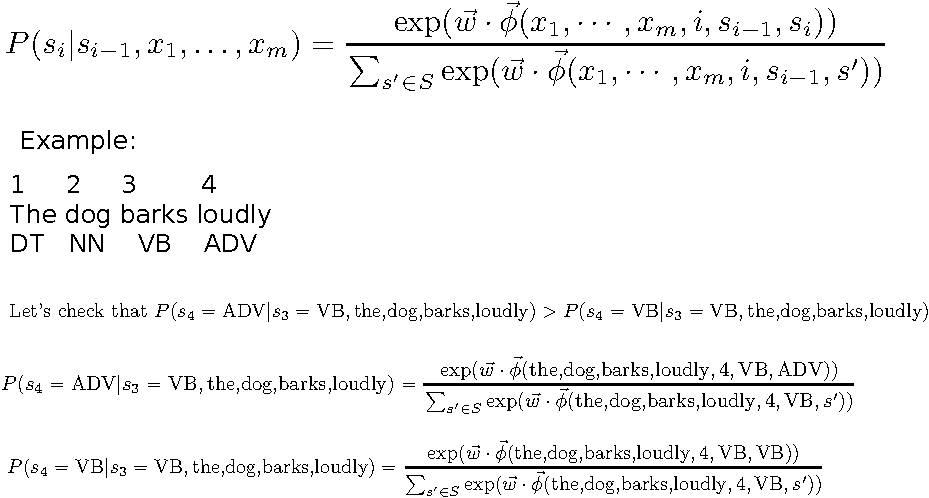
\includegraphics[scale = 0.73]{pics/CRF1.pdf}
        \end{figure}
\end{frame}

\begin{frame}{Example}
  \begin{figure}[h]
        	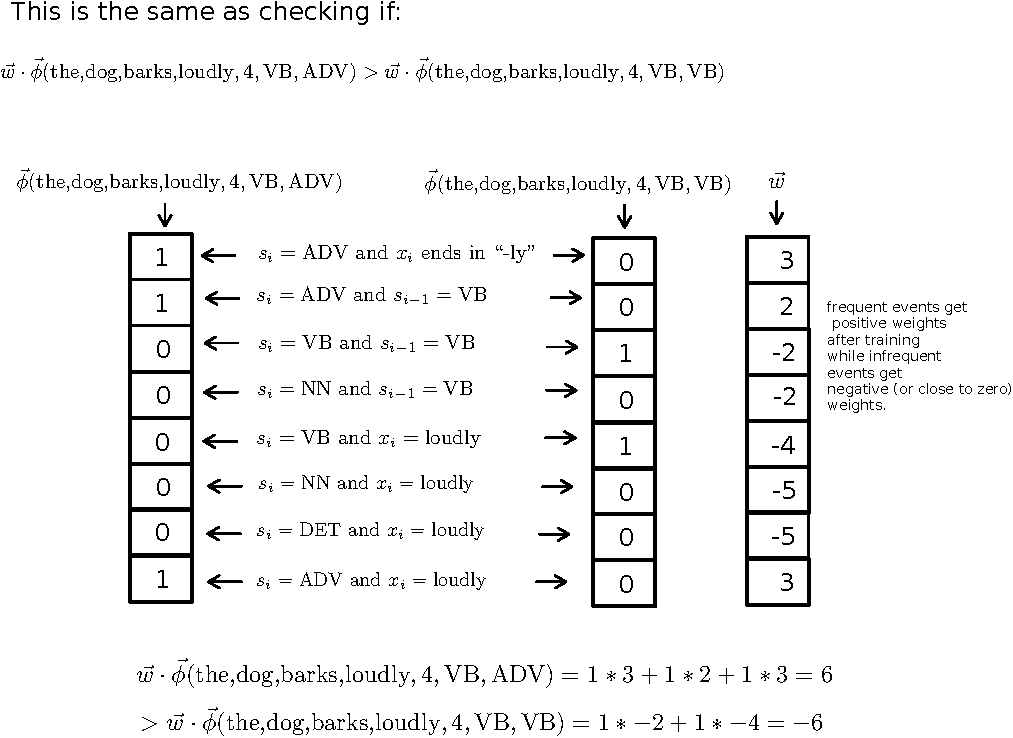
\includegraphics[scale = 0.6]{pics/CRF2.pdf}
        \end{figure}
\end{frame}




\begin{frame}{MEMMs and Multi-class Softmax}
\begin{scriptsize}
\begin{itemize}
\item Notice that the log-linear model from above is very similar to the multi-class softmax model presented in the lecture about linear models.

\item A general log-linear model has the following form:

\begin{displaymath}
 P( y | x; \vec{w}) = \frac{\exp (\vec{w}\cdot \vec{\phi}(x,y))}{\sum_{y' \in Y} \exp (\vec{w}\cdot \vec{\phi}(x,y'))}
\end{displaymath}


\item A multi-class softmax model has the following form:
\begin{equation}
\begin{split}
\hat{\vec{y}} \quad & =  \operatorname{softmax}(\vec{x} \cdot W + \vec{b})  \\
\hat{\vec{y}}_{[i]} \quad & = \frac{e^{(\vec{x} \cdot W + \vec{b})_{[i]}}}{\sum_j e^{(\vec{x} \cdot W + \vec{b})_{[j]}}}
\end{split}
\end{equation}

 
\end{itemize}


\end{scriptsize}
\end{frame}




\begin{frame}{MEMMs and Multi-class Softmax}
\begin{scriptsize}
\begin{itemize}

\item Difference 1: in the log-linear model we have a fixed parameter vector $\vec{w}$ instead of having multiple vectors (one column of $W$ for each class value).

\item Difference 2: the feature vector of the log-linear model $\vec{\phi}(x,y)$ includes information of the label $y$, whereas the input vector $\vec{x}$ of the softmax model is independent of $y$. 

\item Log-linear models allow using features that consider the interaction between $x$ and $y$ (e.g., $x$ ends in ``ly'' and $y$ is an ADVERB).

 
\end{itemize}


\end{scriptsize}
\end{frame}



\begin{frame}{Training MEMMs}
\begin{scriptsize}
\begin{itemize}

\item Once we've defined the feature vectors $\vec{\phi}$, we can train the parameters $\vec{w}$ of the model in the usual way linear models are trained.

\item We set the negative log-likelihood as the loss function and optimize parameters using gradient descent from the training examples.

\item This is equivalent as using the cross-entropy loss.

\item ``Any loss consisting of a negative log-likelihood is a cross-entropy between the empirical distribution defined by the training set and the probability distribution defined by model'' \cite{goodfellow2016deep}.  
 
\end{itemize}


\end{scriptsize}
\end{frame}




\begin{frame}{Decoding with MEMMs}
\begin{scriptsize}
\begin{itemize}

\item The decoding problem is as follows.
\item We are given a new test sequence $x_1, \dots, x_m$.
\item Our goal is to compute the most likely state sequence for this test sequence,

\begin{equation}
 \operatorname{arg} \max_{s_1,\dots,s_m} P(s_1,\dots,s_m|x_1,\dots,x_m).
\end{equation}

\item There are $k^m$ possible state sequences, so for any reasonably large sentence length $m$ brute-force search through all the possibilities will not be possible.

\item We can use the Viterbi alogrithm in a similar way as used for HMMs.
 
\end{itemize}


\end{scriptsize}
\end{frame}



\begin{frame}{Decoding with MEMMs}
\begin{scriptsize}
\begin{itemize}

\item The basic data structure in the algorithm will be a dynamic programming table $\pi$ with entries $\pi[j,s]$ for $j=1, \dots, m$, and $s \in S$.

\item  $\pi[j,s]$ will store the maximum probability for any state sequence ending in state $s$ at position $j$.

\item More formally, our algorithm will compute 
\begin{displaymath}
\pi[j,s] =  \max_{s_1,\dots, s_{j-1}}\left(P(s | s_{j-1}, x_1, \dots, x_m) \prod_{k=1}^{j-1}    P(s_k | s_{k-1}, x_1, \dots, x_m)\right)
\end{displaymath}
for all $j = 1, \dots,m$, and for all $s \in S$.

\end{itemize}


\end{scriptsize}
\end{frame}




\begin{frame}{Decoding with MEMMs}
\begin{scriptsize}
The algorithm is as follows:

\begin{itemize}

\item  Initialization: for $s \in  S$

\begin{displaymath}
  \pi[1,s] = P (s | s_0,x_1,\dots,x_m)
\end{displaymath}
where $s_0$ is a special ``initial'' state.

\item For $j \in \{2,\dots,m\}$, $s \in  \{1,\dots,k\}$

\begin{displaymath}
  \pi[j,s] =  \max_{s' \in S} \ [\pi[j-1,s'] \times P (s | s',x_1,\dots,x_m)]
\end{displaymath}

\end{itemize}



\end{scriptsize}
\end{frame}



\begin{frame}{Decoding with MEMMs}
\begin{scriptsize}

\begin{itemize}

\item  Finally, having filled in the $\pi[j,s]$ values for all $j, s$, we can calculate

\begin{displaymath}
  \max_{s_1,\dots,s_m} = \max_{s} \ \pi[m,s].
\end{displaymath}


\item The algorithm runs in $O(mk^2)$ time (i.e., linear in the sequence length $m$,
and quadratic in the number of tags $k$).


\item As in the Viterbi algorithm for HMMs, we can compute the highest-scoring sequence using backpointers in the dynamic programming algorithm.

\end{itemize}


\end{scriptsize}
\end{frame}


\begin{frame}{Comparison between MEMMs and HMMs}
\begin{scriptsize}

\begin{itemize}

\item  So what is the motivation for using MEMMs instead of HMMs?

\item Note that the Viterbi decoding algorithms for the two models are very similar. 

\item In MEMMs, the probability associated with each state transition $s_{i-1}$ to $s_i$ is

 \begin{displaymath}
 P(s_i | s_{i-1}, x_1, \dots, x_m)  =  \frac{\exp (\vec{w}\cdot \vec{\phi}(x_1, \cdots, x_m, i, s_{i-1},s_i))}{\sum_{s' \in S} \exp (\vec{w}\cdot \vec{\phi}(x_1, \cdots, x_m, i, s_{i-1},s'))}
\end{displaymath}


\item In HMMs, the probability associated with each transition is:

\begin{displaymath}
 P(s_i | s_{i-1}, x_1, \dots, x_m) = P(s_1|s_{i-1})P(x_i|s_i)
\end{displaymath}

\end{itemize}

\end{scriptsize}
\end{frame}



\begin{frame}{Comparison between MEMMs and HMMs}
\begin{scriptsize}

\begin{itemize}

\item  The key advantage of MEMMs is that the use of feature vectors $\vec{\phi}$ allows much
richer representations than those used in HMMs.

\item For example, the transition probability can be sensitive to any word in the input sequence $x_1, \dots, x_m$.

\item In addition, it is very easy to introduce features that are sensitive to spelling features (e.g., prefixes or suffixes) of the current word $x_i$, or of the surrounding words.

\item These features are useful in many NLP applications, and are difficult to incorporate within HMMs in a clean way.

\end{itemize}

\end{scriptsize}
\end{frame}



\begin{frame}{Conditional Random Fields (CRFs)}
\begin{scriptsize}

\begin{itemize}

\item  We now turn to Conditional Random Fields (CRFs) \cite{LaffertyMP01}.

\item Notation: for convenience, we'll use $x_{1:m}$ to refer to an input sequence $x_1 ,\dots,x_m$, and $s_{1:m}$ to refer to a sequence of tags $s_1, \dots, s_m$.

\item The set of all possible tags is again $S$.

\item The set of all possible tag sequences is $S^m$.

\item In conditional random fields we'll again build a model of
\begin{displaymath}
 P(s_1, \dots, s_m | x_1, \dots, x_m) = P(s_{1:m}|x_{1:m})
\end{displaymath}


\end{itemize}

\end{scriptsize}
\end{frame}

\begin{frame}{Conditional Random Fields (CRFs)}
\begin{scriptsize}

\begin{itemize}

\item A first key idea in CRFs will be to define a feature vector  that maps an entire input sequence $x_{1:m}$ paired with an entire tag sequence $s_{1:m}$ to some $d$-dimensional feature vector:

\begin{displaymath}
 \vec{\Phi}(x_{1:m},s_{1:m}) \in \mathcal{R}^d
\end{displaymath}

\item We'll soon give a concrete definition for $\vec{\Phi}$.
\item  For now just assume that some definition exists. 
\item We will often refer to $\vec{\Phi}$ as being a ``global'' feature vector.
\item It is global in the sense that it takes the entire state
sequence into account.

\end{itemize}

\end{scriptsize}
\end{frame}



\begin{frame}{Conditional Random Fields (CRFs)}
\begin{scriptsize}

\begin{itemize}

\item In CRFs we build a giant log-linear model:

\begin{displaymath}
 P(s_{1:m}|x_{1:m}; \vec{w}) = \frac{\exp (\vec{w} \cdot \vec{\Phi}(x_{1:m},s_{1:m}))}{\sum_{s'_{1:m} \in S^m}\exp (\vec{w} \cdot \vec{\Phi}(x_{1:m},s'_{1:m}))}
\end{displaymath}

\item This is ``just'' another log-linear model, but it is is ``giant''.
\item The space of possible values for $s_{1:m}$ is huge $S^m$. 
\item The normalization constant (denominator in the above expression) involves a sum over all possible tag sequences $S^m$.
\item These issues might seem to cause severe computational problems.
\item  Under appropriate assumptions we can train and decode efficiently
with this type of model.
\end{itemize}

\end{scriptsize}
\end{frame}

\begin{frame}{Conditional Random Fields (CRFs)}
\begin{scriptsize}

\begin{itemize}

\item  We define the global feature vector $\vec{\Phi}(x_{1:m},s_{1:m})$ as follows: 

\begin{displaymath}
 \vec{\Phi}(x_{1:m},s_{1:m}) = \sum_{j=1}^{m} \vec{\phi}(x_{1:m},j,s_{j-1},s_j) 
\end{displaymath}

where $\vec{\phi}(x_{1:m},j,s_{j-1},s_j)$ are the same as the feature vectors used in MEMMs.

\item  Example: \ $ \vec{\Phi}([\text{the,dog,barks}],\text{DET,NOUN,VERB}]) = \vec{\phi}([\text{the,dog,barks}],1,*,\text{DET}) + \vec{\phi}([\text{the,dog,barks}],2,\text{DET},\text{NOUN}) + \vec{\phi}([\text{the,dog,barks}],3,\text{NOUN},\text{VERB})$

\item Essentially, we are adding up many sparse vectors.



\end{itemize}



\end{scriptsize}
\end{frame}


\begin{frame}{Example}
  \begin{figure}[h]
        	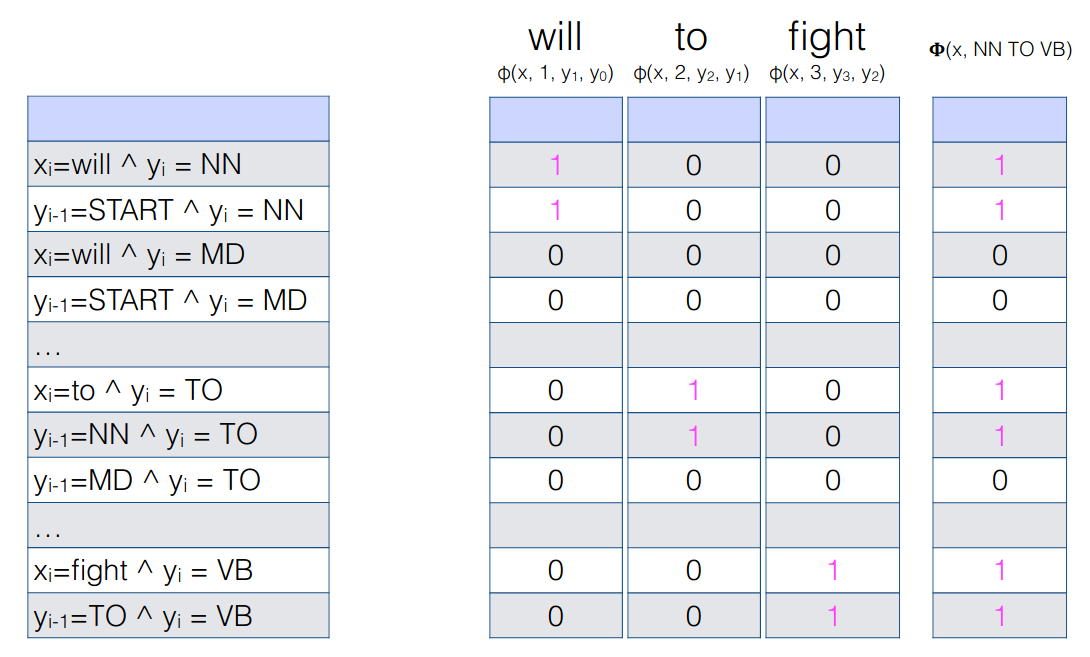
\includegraphics[scale = 0.26]{pics/CRF3.png}
        \end{figure}
        
        \footnotemark{source: \url{http://people.ischool.berkeley.edu/~dbamman/nlpF18/slides/12_neural_sequence_labeling.pdf}}
\end{frame}


\begin{frame}{Conditional Random Fields (CRFs)}
\begin{scriptsize}

\begin{itemize}
\item We are assuming that for any dimension of $\vec{\Phi}_{[k]}, k= 1, \dots, d$, the $k$'th global feature is:

\begin{displaymath}
 \vec{\Phi}(x_{1:m},s_{1:m})_{[k]} = \sum_{j=1}^{m} \vec{\phi}(x_{1:m},j,s_{j-1},s_j)_{[k]} 
\end{displaymath}

\item Thus $\vec{\Phi}(x_{1:m},s_{1:m})_{[k]}$ is calculated by summing the ``local'' feature vector $\vec{\phi}(x_{1:m},j,s_{j-1},s_j)_{[k]}$  over the m different tag transitions in $s_1,\dots,s_m$.


\item We would expect each local vector to encode relevant information about the tag transition by turning on some vector dimensions (setting the value to one).

\item We now turn to two critical practical issues in CRFs: first, decoding, and sec-
ond, parameter estimation (training).

\end{itemize}

\end{scriptsize}
\end{frame}



\begin{frame}{Decoding with CRFs}
\begin{scriptsize}

\begin{itemize}
\item The decoding problem in CRFs is as follows.
\item For a given input sequence $x_{1:m} = x_1 , x_2 , \dots, x_m$ , we would like to find the most likely underlying  state sequence under the model, that is,

\begin{equation}
 \begin{split}
 arg \max_{s_{1:m} \in S^m} P(s_{1:m}| x_{1:m}; \vec{w})  \quad & =  arg \max_{s_{1:m} \in S^m} \frac{\exp (\vec{w} \cdot \vec{\Phi}(x_{1:m},s_{1:m}))}{\sum_{s'_{1:m} \in S^m}\exp (\vec{w} \cdot \vec{\Phi}(x_{1:m},s'_{1:m}))} \\
 \quad & =  arg \max_{s_{1:m} \in S^m} \exp (\vec{w} \cdot \vec{\Phi}(x_{1:m},s_{1:m})) \\
  \quad & =  arg \max_{s_{1:m} \in S^m}  \vec{w} \cdot \vec{\Phi}(x_{1:m},s_{1:m}) \\
    \quad & =  arg \max_{s_{1:m} \in S^m}  \vec{w} \cdot \sum_{j=1}^{m} \vec{\phi}(x_{1:m},j,s_{j-1},s_j) \\
 \quad & =  arg \max_{s_{1:m} \in S^m}  \sum_{j=1}^{m} \vec{w} \cdot \vec{\phi}(x_{1:m},j,s_{j-1},s_j)   
 \end{split}
 \end{equation}




\end{itemize}

\end{scriptsize}
\end{frame}



\begin{frame}{Decoding with CRFs}
\begin{scriptsize}

\begin{itemize}
\item We have shown that finding the most likely sequence under the model is equivalent to finding the sequence that maximizes:

\begin{displaymath}
 arg \max_{s_{1:m} \in S^m}  \sum_{j=1}^{m} \vec{w} \cdot \vec{\phi}(x_{1:m},j,s_{j-1},s_j)  
\end{displaymath}

\item This problem has a clear intuition. Each transition from tag  $s_{j-1}$ to tag $s_j$ has an associated score:  $\vec{w} \cdot \vec{\phi}(x_{1:m},j,s_{j-1},s_j)$  


\item This score could be positive or negative. 

\item Intuitively, this score will be relatively high if the state transition is plausible, relatively low if this transition is implausible.

\item  The decoding problem is to find an entire sequence of states such that the sum of transition scores is maximized.

\item We can again solve this problem using a variant of the Viterbi algorithm, in a very similar way to the decoding algorithm for HMMs or MEMMs.

\end{itemize}


\end{scriptsize}
\end{frame}



\begin{frame}{Parameter Estimation in CRFs (training)}
\begin{scriptsize}

\begin{itemize}
\item For parameter estimation, we assume we have a set of $n$ labeled examples, $\{(x_{1:m}^i, s_{1:m}^i )\}_{i=1}^n$ . Each $x_{1:m}^i$ is an input sequence $x_1^i, \dots , x_m^i$ each $s_{1:m}^i$ is a tag sequence $s_1^i, \dots , s_m^i$.

\item We again set the negative log-likelihood (or cross-entropy) as the loss function $L$ as optimize parameters using gradient descent.

\item The main challenge here is that gradient calculations $\frac{\partial L}{\partial \vec{w}_{[k]}}$ involve summing over $S^m$ (a very large set containing all possible tag sequences).

\item This sum can be computed efficiently using the Forward-backward algorithm\footnote{\url{http://www.cs.columbia.edu/~mcollins/fb.pdf}}. 

\item This is another dynamic programming algorithm that is closely related
to the Viterbi algorithm.

\end{itemize}


\end{scriptsize}
\end{frame}



\begin{frame}{CRFs and MEMMs}
\begin{scriptsize}

\begin{itemize}

\item CRFs and MEMMS are discriminative sequence labeling models: they model the conditional probability directly via a parameterized log-linear multi-class function (softmax).

\item HMMs, on the other hand, are generative models.

\item In MEMM the normalization (denominator of the softmax) is local: it happens at each tag step (the sum runs over all possible tag values $S$).

\item In CRFs the normalization is global: the sum runs over all possible tag sequences $S^m$.

\item Training a MEMM is quite easy: just train a multi-class log-linear model for for a given word to the label. This classifier is used at each word step to predict the whole sequence.

\item Training CRF is more complex. The objective  is to maximize the log probability of the most likely sequence.


\end{itemize}

\end{scriptsize}
\end{frame}




\begin{frame}{CRFs and MEMMs: the label bias problem}
\begin{scriptsize}

\begin{itemize}

\item MEMMs end up making up decision at each time step independently.

\item This leads to a problem called label bias: in some tag space configurations, MEMMs essentially completely ignore important aspects of the context.

\item Example: The right POS labeling of sentence ``will to fight'' (la voluntad de pelear) is ``NN TO VB''. \footnote{Here we are using the PENN Treebank tagset: \url{https://www.eecis.udel.edu/~vijay/cis889/ie/pos-set.pdf}} 

\item Here NN stands for ``noun'', TO stands for ``infinitive to'',  and VB stands for ``verb base form''.

\item Modals (MD) show up much more frequently at the start of the sentence than nouns do (e.g., questions).

\item Hence, tag ``MD'' will receive a higher score than tag ``NN'' when $x_0$=``will'' : $P(s_1 = MD|s_{0} = *,x_1 = \text{``will''},...) > P( s_1 = NN| s_{i-1} = *, x_1 = \text{``will''})$.


\item But we know that MD + TO is very rare: ``... can to eat'', ``... would to eat''.



\end{itemize}

\end{scriptsize}
\end{frame}




\begin{frame}{CRFs and MEMMs: the label bias problem}
\begin{scriptsize}

\begin{itemize}

\item The word ``to'' is relatively deterministic (almost always has tag TO) so it doesn't matter what tag precedes it.

\item Because of the local normalization of MEMMs, $P(s_i = TO | s_{i-1}, x_1, \dots, x_i = \text{``to''}, \dots, x_n)$ will always be 1 when $x_i=$``to'' regardless of the value of $s_{i-1}$ (MD or NN).

\item That means our prediction for ``to'' can't help us disambiguate ``will''.  

\item We lose the information that MD + TO sequences rarely happen.

\item As a consequence: a MEMMS would likely label the first word to ``MD''.

\item CRF overcomes this issue by doing a global normalization: it considers the score of the whole sequence before normalizing to make it a probability distribution.



\end{itemize}

\end{scriptsize}
\end{frame}


% Label Bias•In some state space configurations,MEMMs essentially completely ignore the inputs.•Example (ON BOARD)
% "label bias problem," where states with low-entropy transition distributions "effectively ignore their observations."
% These are names for situations when one source of information is ignored because it isexplained away by anothersource

\begin{frame}{Links}
\begin{scriptsize}
\begin{itemize}

\item \url{http://people.ischool.berkeley.edu/~dbamman/nlpF18/slides/11_memm_crf.pdf}

\item \url{http://people.ischool.berkeley.edu/~dbamman/nlpF18/slides/12_neural_sequence_labeling.pdf}

\item \url{https://www.depends-on-the-definition.com/sequence-tagging-lstm-crf/}

\item \url{https://www.quora.com/What-are-the-pros-and-cons-of-these-three-sequence-models-MaxEnt-Markov-Model-Conditional-random-fields-and-recurrent-neural-networks}

\item \url{https://people.cs.umass.edu/~mccallum/papers/crf-tutorial.pdf}

\item \url{http://www.davidsbatista.net/blog/2017/11/13/Conditional_Random_Fields} 

\end{itemize}


\end{scriptsize}
\end{frame}






\begin{frame}
\frametitle{Questions?}
%\vspace{1.5cm}
\begin{center}\LARGE Thanks for your Attention!\\ \end{center}



\end{frame}

\begin{frame}[allowframebreaks]\scriptsize
\frametitle{References}
\bibliography{bio}
\bibliographystyle{apalike}
%\bibliographystyle{flexbib}
\end{frame}  


%%%%%%%%%%%%%%%%%%%%%%%%%%%

\end{document}
